\documentclass[11pt]{article}
\usepackage[margin=1in]{geometry}
\usepackage[T1]{fontenc}
\usepackage{lmodern}
\usepackage{amsmath,amssymb}
\usepackage{graphicx}
\usepackage{booktabs}
\usepackage{caption}
\usepackage{microtype}
\usepackage[numbers,sort&compress]{natbib}
\usepackage{tikz}
\usetikzlibrary{positioning,arrows.meta}
\usepackage[colorlinks=true,linkcolor=blue!50!black,citecolor=blue!50!black,urlcolor=blue!50!black]{hyperref}
\usepackage{cleveref}

\captionsetup{font=small,labelfont=bf}
\graphicspath{{figures/}}
% Auto-generated by scripts/make_macros.py -- do not edit.
\newcommand{\DataAssets}{417}
\newcommand{\DataDays}{3{,}772}
\newcommand{\DataStart}{January 2010}
\newcommand{\DataEnd}{December 2024}
\newcommand{\NEpisodes}{168}
\newcommand{\MinTrain}{24}
\newcommand{\OOSStart}{7 January 2013}
\newcommand{\FullOverlap}{0.984}
\newcommand{\FullLamZero}{161}
\newcommand{\FullLamZeroShare}{39}
\newcommand{\RollMPUpper}{5.23}
\newcommand{\RollQ}{1.65}
\newcommand{\FullNSigRescaled}{36}
\newcommand{\SRMarketLevel}{$-$0.09}
\newcommand{\TMarketLevel}{$-$0.33}
\newcommand{\SRMarketRet}{0.18}
\newcommand{\TMarketRet}{0.56}
\newcommand{\ACMarket}{$-$0.066}
\newcommand{\ACtMarket}{$-$4.1}
\newcommand{\SRSignalLevel}{0.07}
\newcommand{\TSignalLevel}{0.26}
\newcommand{\SRSignalRet}{$-$0.57}
\newcommand{\TSignalRet}{$-$1.96}
\newcommand{\ACSignal}{$-$0.047}
\newcommand{\ACtSignal}{$-$6.3}
\newcommand{\SREdgeLevel}{$-$0.00}
\newcommand{\TEdgeLevel}{$-$0.02}
\newcommand{\SREdgeRet}{$-$0.25}
\newcommand{\TEdgeRet}{$-$0.71}
\newcommand{\ACEdge}{$-$0.054}
\newcommand{\ACtEdge}{$-$12.0}
\newcommand{\SRUpperLevel}{0.54}
\newcommand{\TUpperLevel}{1.86}
\newcommand{\SRUpperRet}{0.63}
\newcommand{\TUpperRet}{2.89}
\newcommand{\ACUpper}{$-$0.057}
\newcommand{\ACtUpper}{$-$21.7}
\newcommand{\SRMiddleLevel}{0.87}
\newcommand{\TMiddleLevel}{2.74}
\newcommand{\SRMiddleRet}{1.10}
\newcommand{\TMiddleRet}{4.07}
\newcommand{\ACMiddle}{$-$0.057}
\newcommand{\ACtMiddle}{$-$21.7}
\newcommand{\SRLowerLevel}{0.70}
\newcommand{\TLowerLevel}{2.39}
\newcommand{\SRLowerRet}{0.95}
\newcommand{\TLowerRet}{3.14}
\newcommand{\ACLower}{$-$0.056}
\newcommand{\ACtLower}{$-$22.1}
\newcommand{\OUSlope}{$-$0.14}
\newcommand{\OUSpearman}{$-$0.30}
\newcommand{\OUNoRev}{10}
\newcommand{\CalmVol}{10}
\newcommand{\StressVol}{22}
\newcommand{\CalmCorr}{0.25}
\newcommand{\StressCorr}{0.52}
\newcommand{\PStayCalm}{0.991}
\newcommand{\PStayStress}{0.981}
\newcommand{\FracStress}{29}
\newcommand{\StressTwentyTwenty}{78}
\newcommand{\StressTwentyTwentyTwo}{92}
\newcommand{\StressTwentySeventeen}{0}
\newcommand{\BaseRateA}{62}
\newcommand{\OOSRowsA}{4{,}320}
\newcommand{\AUCLogitModeA}{0.523}
\newcommand{\AUCLoLogitModeA}{0.506}
\newcommand{\AUCHiLogitModeA}{0.540}
\newcommand{\AUCLogitAllA}{0.521}
\newcommand{\AUCLoLogitAllA}{0.501}
\newcommand{\AUCHiLogitAllA}{0.537}
\newcommand{\AUCGbmModeA}{0.518}
\newcommand{\AUCLoGbmModeA}{0.502}
\newcommand{\AUCHiGbmModeA}{0.535}
\newcommand{\AUCGbmAllA}{0.518}
\newcommand{\AUCLoGbmAllA}{0.499}
\newcommand{\AUCHiGbmAllA}{0.538}
\newcommand{\AUCRfModeA}{0.524}
\newcommand{\AUCLoRfModeA}{0.508}
\newcommand{\AUCHiRfModeA}{0.543}
\newcommand{\AUCRfAllA}{0.528}
\newcommand{\AUCLoRfAllA}{0.509}
\newcommand{\AUCHiRfAllA}{0.545}
\newcommand{\AUCHeurHalfLifeA}{0.512}
\newcommand{\AUCHeurLambdaA}{0.504}
\newcommand{\BaseRateB}{62}
\newcommand{\OOSRowsB}{35{,}856}
\newcommand{\AUCLogitModeB}{0.508}
\newcommand{\AUCLoLogitModeB}{0.500}
\newcommand{\AUCHiLogitModeB}{0.515}
\newcommand{\AUCLogitAllB}{0.514}
\newcommand{\AUCLoLogitAllB}{0.505}
\newcommand{\AUCHiLogitAllB}{0.522}
\newcommand{\AUCGbmModeB}{0.506}
\newcommand{\AUCLoGbmModeB}{0.501}
\newcommand{\AUCHiGbmModeB}{0.512}
\newcommand{\AUCGbmAllB}{0.504}
\newcommand{\AUCLoGbmAllB}{0.497}
\newcommand{\AUCHiGbmAllB}{0.512}
\newcommand{\AUCRfModeB}{0.507}
\newcommand{\AUCLoRfModeB}{0.500}
\newcommand{\AUCHiRfModeB}{0.513}
\newcommand{\AUCRfAllB}{0.512}
\newcommand{\AUCLoRfAllB}{0.505}
\newcommand{\AUCHiRfAllB}{0.520}
\newcommand{\AUCHeurHalfLifeB}{0.512}
\newcommand{\AUCHeurLambdaB}{0.493}
\newcommand{\BaseRateACalm}{61}
\newcommand{\AUCRegACalm}{0.509}
\newcommand{\NEpACalm}{102}
\newcommand{\BaseRateAStress}{65}
\newcommand{\AUCRegAStress}{0.522}
\newcommand{\NEpAStress}{42}
\newcommand{\BaseRateBCalm}{62}
\newcommand{\AUCRegBCalm}{0.510}
\newcommand{\NEpBCalm}{102}
\newcommand{\BaseRateBStress}{64}
\newcommand{\AUCRegBStress}{0.507}
\newcommand{\NEpBStress}{42}
\newcommand{\SREWA}{$-$0.20}
\newcommand{\GSREWA}{0.16}
\newcommand{\RetEWA}{$-$0.8}
\newcommand{\GRetEWA}{0.6}
\newcommand{\VolEWA}{3.8}
\newcommand{\DDEWA}{$-$22.7}
\newcommand{\TOEWA}{0.27}
\newcommand{\BEEWA}{0.88}
\newcommand{\CorrEWA}{0.31}
\newcommand{\SRMPA}{$-$0.14}
\newcommand{\GSRMPA}{0.11}
\newcommand{\RetMPA}{$-$0.7}
\newcommand{\GRetMPA}{0.6}
\newcommand{\VolMPA}{5.2}
\newcommand{\DDMPA}{$-$20.2}
\newcommand{\TOMPA}{0.26}
\newcommand{\BEMPA}{0.88}
\newcommand{\CorrMPA}{0.18}
\newcommand{\SRHeurA}{$-$0.46}
\newcommand{\GSRHeurA}{0.14}
\newcommand{\RetHeurA}{$-$1.1}
\newcommand{\GRetHeurA}{0.4}
\newcommand{\VolHeurA}{2.5}
\newcommand{\DDHeurA}{$-$15.1}
\newcommand{\TOHeurA}{0.30}
\newcommand{\BEHeurA}{0.47}
\newcommand{\CorrHeurA}{0.22}
\newcommand{\SRMLModeA}{$-$0.29}
\newcommand{\GSRMLModeA}{0.24}
\newcommand{\RetMLModeA}{$-$0.8}
\newcommand{\GRetMLModeA}{0.7}
\newcommand{\VolMLModeA}{2.7}
\newcommand{\DDMLModeA}{$-$15.7}
\newcommand{\TOMLModeA}{0.29}
\newcommand{\BEMLModeA}{0.91}
\newcommand{\CorrMLModeA}{0.22}
\newcommand{\SRMLAllA}{$-$0.50}
\newcommand{\GSRMLAllA}{0.07}
\newcommand{\RetMLAllA}{$-$1.3}
\newcommand{\GRetMLAllA}{0.2}
\newcommand{\VolMLAllA}{2.5}
\newcommand{\DDMLAllA}{$-$15.2}
\newcommand{\TOMLAllA}{0.29}
\newcommand{\BEMLAllA}{0.25}
\newcommand{\CorrMLAllA}{0.23}
\newcommand{\SRMLOverA}{$-$0.21}
\newcommand{\GSRMLOverA}{0.18}
\newcommand{\RetMLOverA}{$-$0.4}
\newcommand{\GRetMLOverA}{0.4}
\newcommand{\VolMLOverA}{2.0}
\newcommand{\DDMLOverA}{$-$9.2}
\newcommand{\TOMLOverA}{0.15}
\newcommand{\BEMLOverA}{0.93}
\newcommand{\CorrMLOverA}{0.23}
\newcommand{\SREWOverA}{$-$0.09}
\newcommand{\GSREWOverA}{0.14}
\newcommand{\RetEWOverA}{$-$0.3}
\newcommand{\GRetEWOverA}{0.5}
\newcommand{\VolEWOverA}{3.2}
\newcommand{\DDEWOverA}{$-$14.4}
\newcommand{\TOEWOverA}{0.14}
\newcommand{\BEEWOverA}{1.26}
\newcommand{\CorrEWOverA}{0.29}
\newcommand{\SREWB}{$-$0.14}
\newcommand{\GSREWB}{0.81}
\newcommand{\RetEWB}{$-$0.3}
\newcommand{\GRetEWB}{1.8}
\newcommand{\VolEWB}{2.2}
\newcommand{\DDEWB}{$-$10.7}
\newcommand{\TOEWB}{0.42}
\newcommand{\BEEWB}{1.70}
\newcommand{\CorrEWB}{0.36}
\newcommand{\SRHeurB}{$-$0.67}
\newcommand{\GSRHeurB}{0.67}
\newcommand{\RetHeurB}{$-$1.1}
\newcommand{\GRetHeurB}{1.1}
\newcommand{\VolHeurB}{1.6}
\newcommand{\DDHeurB}{$-$13.0}
\newcommand{\TOHeurB}{0.43}
\newcommand{\BEHeurB}{1.00}
\newcommand{\CorrHeurB}{0.31}
\newcommand{\SRMLModeB}{$-$0.25}
\newcommand{\GSRMLModeB}{0.74}
\newcommand{\RetMLModeB}{$-$0.5}
\newcommand{\GRetMLModeB}{1.4}
\newcommand{\VolMLModeB}{1.9}
\newcommand{\DDMLModeB}{$-$11.6}
\newcommand{\TOMLModeB}{0.37}
\newcommand{\BEMLModeB}{1.50}
\newcommand{\CorrMLModeB}{0.30}
\newcommand{\SRMLAllB}{$-$0.12}
\newcommand{\GSRMLAllB}{0.85}
\newcommand{\RetMLAllB}{$-$0.2}
\newcommand{\GRetMLAllB}{1.6}
\newcommand{\VolMLAllB}{1.9}
\newcommand{\DDMLAllB}{$-$10.8}
\newcommand{\TOMLAllB}{0.36}
\newcommand{\BEMLAllB}{1.76}
\newcommand{\CorrMLAllB}{0.29}
\newcommand{\SRMLOverB}{0.19}
\newcommand{\GSRMLOverB}{0.95}
\newcommand{\RetMLOverB}{0.3}
\newcommand{\GRetMLOverB}{1.5}
\newcommand{\VolMLOverB}{1.6}
\newcommand{\DDMLOverB}{$-$6.7}
\newcommand{\TOMLOverB}{0.24}
\newcommand{\BEMLOverB}{2.49}
\newcommand{\CorrMLOverB}{0.30}
\newcommand{\SREWOverB}{0.16}
\newcommand{\GSREWOverB}{0.89}
\newcommand{\RetEWOverB}{0.3}
\newcommand{\GRetEWOverB}{1.7}
\newcommand{\VolEWOverB}{1.9}
\newcommand{\DDEWOverB}{$-$6.2}
\newcommand{\TOEWOverB}{0.28}
\newcommand{\BEEWOverB}{2.44}
\newcommand{\CorrEWOverB}{0.37}
\newcommand{\SROrig}{$-$1.53}
\newcommand{\GSROrig}{$-$0.53}
\newcommand{\TOOrig}{1.36}
\newcommand{\DDOrig}{$-$126}
\newcommand{\BEOrig}{$-$1.06}
\newcommand{\PlaceboMeanA}{$-$0.37}
\newcommand{\PlaceboNFA}{$-$0.07}
\newcommand{\PlaceboPMLModeA}{0.310}
\newcommand{\PlaceboPMLAllA}{0.755}
\newcommand{\DiffHeurA}{$-$0.26}
\newcommand{\DiffPHeurA}{0.85}
\newcommand{\DiffMLModeA}{$-$0.09}
\newcommand{\DiffPMLModeA}{0.69}
\newcommand{\DiffMLAllA}{$-$0.30}
\newcommand{\DiffPMLAllA}{0.95}
\newcommand{\DiffMLOverA}{$-$0.01}
\newcommand{\DiffPMLOverA}{0.50}
\newcommand{\DiffEWOverA}{$+$0.12}
\newcommand{\DiffPEWOverA}{0.16}
\newcommand{\MeanExpA}{0.52}
\newcommand{\MinExpA}{0.00}
\newcommand{\MeanExpEWA}{0.52}
\newcommand{\PlaceboMeanB}{$-$0.71}
\newcommand{\PlaceboNFB}{$-$0.46}
\newcommand{\PlaceboPMLModeB}{0.000}
\newcommand{\PlaceboPMLAllB}{0.000}
\newcommand{\DiffHeurB}{$-$0.52}
\newcommand{\DiffPHeurB}{1.00}
\newcommand{\DiffMLModeB}{$-$0.10}
\newcommand{\DiffPMLModeB}{0.72}
\newcommand{\DiffMLAllB}{$+$0.03}
\newcommand{\DiffPMLAllB}{0.46}
\newcommand{\DiffMLOverB}{$+$0.33}
\newcommand{\DiffPMLOverB}{0.09}
\newcommand{\DiffEWOverB}{$+$0.31}
\newcommand{\DiffPEWOverB}{0.01}
\newcommand{\MeanExpB}{0.65}
\newcommand{\MinExpB}{0.18}
\newcommand{\MeanExpEWB}{0.64}
\newcommand{\RegSREWACalm}{$-$0.67}
\newcommand{\RegSREWAStress}{0.31}
\newcommand{\RegSREWOverACalm}{$-$0.87}
\newcommand{\RegSREWOverAStress}{0.41}
\newcommand{\RegSRMLAllACalm}{$-$1.12}
\newcommand{\RegSRMLAllAStress}{0.34}
\newcommand{\RegSRMLOverACalm}{$-$1.04}
\newcommand{\RegSRMLOverAStress}{0.36}
\newcommand{\RegSREWBCalm}{$-$1.05}
\newcommand{\RegSREWBStress}{0.79}
\newcommand{\RegSREWOverBCalm}{$-$0.74}
\newcommand{\RegSREWOverBStress}{0.79}
\newcommand{\RegSRMLAllBCalm}{$-$0.72}
\newcommand{\RegSRMLAllBStress}{0.65}
\newcommand{\RegSRMLOverBCalm}{$-$0.45}
\newcommand{\RegSRMLOverBStress}{0.74}
\newcommand{\SRCostZeroEWA}{0.16}
\newcommand{\SRCostZeroHeurA}{0.14}
\newcommand{\SRCostZeroMLAllA}{0.07}
\newcommand{\SRCostFiveEWA}{$-$0.74}
\newcommand{\SRCostFiveHeurA}{$-$1.37}
\newcommand{\SRCostFiveMLAllA}{$-$1.35}
\newcommand{\SRCostTenEWA}{$-$1.63}
\newcommand{\SRCostTenHeurA}{$-$2.85}
\newcommand{\SRCostTenMLAllA}{$-$2.75}
\newcommand{\SRCostZeroEWB}{0.81}
\newcommand{\SRCostZeroHeurB}{0.67}
\newcommand{\SRCostZeroMLAllB}{0.85}
\newcommand{\SRCostFiveEWB}{$-$1.57}
\newcommand{\SRCostFiveHeurB}{$-$2.65}
\newcommand{\SRCostFiveMLAllB}{$-$1.56}
\newcommand{\SRCostTenEWB}{$-$3.91}
\newcommand{\SRCostTenHeurB}{$-$5.85}
\newcommand{\SRCostTenMLAllB}{$-$3.91}
\newcommand{\RobSubperiodTwoZeroOneThreeTwoZeroOneSixMLA}{$-$1.27}
\newcommand{\RobSubperiodTwoZeroOneThreeTwoZeroOneSixEWA}{$-$0.92}
\newcommand{\RobSubperiodTwoZeroOneSevenTwoZeroOneNineMLA}{$-$0.20}
\newcommand{\RobSubperiodTwoZeroOneSevenTwoZeroOneNineEWA}{$-$0.29}
\newcommand{\RobSubperiodTwoZeroTwoZeroTwoZeroTwoOneMLA}{$-$0.05}
\newcommand{\RobSubperiodTwoZeroTwoZeroTwoZeroTwoOneEWA}{0.30}
\newcommand{\RobSubperiodTwoZeroTwoTwoTwoZeroTwoFourMLA}{$-$0.65}
\newcommand{\RobSubperiodTwoZeroTwoTwoTwoZeroTwoFourEWA}{$-$0.19}
\newcommand{\RobSubperiodTwoZeroOneThreeTwoZeroOneSixMLB}{0.04}
\newcommand{\RobSubperiodTwoZeroOneThreeTwoZeroOneSixEWB}{0.04}
\newcommand{\RobSubperiodTwoZeroOneSevenTwoZeroOneNineMLB}{$-$0.74}
\newcommand{\RobSubperiodTwoZeroOneSevenTwoZeroOneNineEWB}{$-$0.34}
\newcommand{\RobSubperiodTwoZeroTwoZeroTwoZeroTwoOneMLB}{0.44}
\newcommand{\RobSubperiodTwoZeroTwoZeroTwoZeroTwoOneEWB}{0.56}
\newcommand{\RobSubperiodTwoZeroTwoTwoTwoZeroTwoFourMLB}{$-$0.49}
\newcommand{\RobSubperiodTwoZeroTwoTwoTwoZeroTwoFourEWB}{$-$1.20}
\newcommand{\RobSelecttopTwoZeropctMLA}{$-$0.63}
\newcommand{\RobSelecttopTwoZeropctEWA}{$-$0.20}
\newcommand{\RobSelecttopFiveZeropctMLA}{$-$0.42}
\newcommand{\RobSelecttopFiveZeropctEWA}{$-$0.20}
\newcommand{\RobModelGBMMLA}{$-$0.65}
\newcommand{\RobModelGBMEWA}{$-$0.20}
\newcommand{\RobModelRFMLA}{$-$0.36}
\newcommand{\RobModelRFEWA}{$-$0.20}
\newcommand{\RobSelecttopTwoZeropctMLB}{$-$0.25}
\newcommand{\RobSelecttopTwoZeropctEWB}{$-$0.14}
\newcommand{\RobSelecttopFiveZeropctMLB}{$-$0.08}
\newcommand{\RobSelecttopFiveZeropctEWB}{$-$0.14}
\newcommand{\RobModelGBMMLB}{$-$0.56}
\newcommand{\RobModelGBMEWB}{$-$0.14}
\newcommand{\RobModelRFMLB}{$-$0.54}
\newcommand{\RobModelRFEWB}{$-$0.14}
\newcommand{\RobExecutiondelaypOnedayMLA}{$-$0.53}
\newcommand{\RobExecutiondelaypOnedayEWA}{$-$0.27}
\newcommand{\RobExecutiondelaypOnedayMLB}{$-$0.74}
\newcommand{\RobExecutiondelaypOnedayEWB}{$-$0.59}
\newcommand{\RobWindowWOneTwoSixMLA}{$-$0.60}
\newcommand{\RobWindowWOneTwoSixEWA}{$-$0.24}
\newcommand{\RobWindowWOneTwoSixMLB}{$-$0.63}
\newcommand{\RobWindowWOneTwoSixEWB}{$-$0.28}
\newcommand{\RobWindowWFiveZeroFourMLA}{$-$0.58}
\newcommand{\RobWindowWFiveZeroFourEWA}{$-$0.10}
\newcommand{\RobWindowWFiveZeroFourMLB}{$-$0.13}
\newcommand{\RobWindowWFiveZeroFourEWB}{$-$0.31}
\newcommand{\RobLookbackLTwoZeroMLA}{$-$0.70}
\newcommand{\RobLookbackLTwoZeroEWA}{$-$0.43}
\newcommand{\RobLookbackLTwoZeroMLB}{$-$0.97}
\newcommand{\RobLookbackLTwoZeroEWB}{$-$0.36}
\newcommand{\RobLookbackLOneTwoZeroMLA}{$-$0.66}
\newcommand{\RobLookbackLOneTwoZeroEWA}{$-$0.21}
\newcommand{\RobLookbackLOneTwoZeroMLB}{$-$0.82}
\newcommand{\RobLookbackLOneTwoZeroEWB}{$-$0.13}
\newcommand{\RobHoldingHOneZeroMLA}{$-$0.31}
\newcommand{\RobHoldingHOneZeroEWA}{$-$0.07}
\newcommand{\RobHoldingHOneZeroMLB}{$-$1.22}
\newcommand{\RobHoldingHOneZeroEWB}{$-$0.44}
\newcommand{\RobHoldingHFourTwoMLA}{$-$0.35}
\newcommand{\RobHoldingHFourTwoEWA}{$-$0.26}
\newcommand{\RobHoldingHFourTwoMLB}{$-$0.24}
\newcommand{\RobHoldingHFourTwoEWB}{$-$0.12}


\title{Normal Modes of the Market:\\
Mean Reversion Across the Correlation Spectrum,\\
Machine-Learned Mode Selection, and Regimes}
\author{Besufikad\thanks{University of Chicago. Code and data pipeline:
\url{https://github.com/besufikad-a/normal-modes-of-the-market}.}}
\date{Working paper --- October 2026}

\begin{document}
\maketitle

\begin{abstract}
\noindent
We test whether the normal modes of the U.S. equity correlation matrix
exhibit predictable mean reversion. In the overdamped limit of a
coupled-oscillator market, the covariance matrix is the inverse of the
stiffness matrix, so the lowest-variance eigenportfolios should relax
fastest. Using \DataAssets{} S\&P~500 stocks, monthly walk-forward
re-estimation and out-of-sample data from 2013 to 2024, we find that the
modes the Marchenko--Pastur filter certifies as signal do not revert
(Sharpe \SRSignalLevel), while modes deep in the noise bulk do (Sharpe
up to \SRMiddleLevel, $t=\TMiddleLevel$), with significantly negative
daily autocorrelation. Supervised models using eigenvalue separation,
half-life, autocorrelation, eigenvector stability, volatility,
portfolio concentration and regime features predict which modes will
revert with out-of-sample AUC of 0.51--0.53: significant, and better
than random selection, but not better than holding every mode. A
two-state hidden Markov model reveals a strong regime asymmetry:
reversion profits arise in high-volatility, high-correlation states and
reverse in calm ones. A walk-forward strategy combining mode
predictions with regime-based exposure reaches a net Sharpe ratio of
\SRMLOverB{} at 2~bp costs. That result depends on same-close execution
and on an overlay whose form was chosen after observing the regime
asymmetry. Overall, the normal-mode picture locates mean reversion
correctly in the spectrum, but after costs, and once the specifications
we tried are taken into account, it provides little tradable alpha.
\end{abstract}

\section{Introduction}

A system of coupled harmonic oscillators decomposes into normal modes:
orthogonal coordinates that evolve independently, each with its own
characteristic frequency. The eigen-decomposition of an equity
correlation matrix has the same algebraic form. Its eigenvectors are
portfolios with (in-sample) uncorrelated returns, and its eigenvalues
are their variances. This paper asks whether the analogy can be made
\emph{predictive}. Do some normal modes of the market behave like
displaced oscillators that are pulled back to equilibrium, and can we
tell in advance which ones?

The question connects three literatures. Random matrix theory shows
that most of the eigenvalues of a large sample correlation matrix are
indistinguishable from noise, and the Marchenko--Pastur law gives a
principled edge between signal and noise
\citep{laloux1999,plerou2002,bunbouchaud2017}. Statistical arbitrage
trades the mean reversion of residual portfolios, typically residuals
of stocks against principal-component or ETF factors
\citep{avellaneda2010,gatev2006}, and short-term reversal profits are
known to vary strongly with market conditions
\citep{lehmann1990,nagel2012,khandani2011}. Machine-learning methods
have become a standard tool for extracting weak predictive signals from
many correlated characteristics \citep{gu2020}.

We make three contributions.

\emph{A physical prediction and a spectrum-wide test.} We take the
oscillator analogy to its overdamped, thermally driven limit, a
multivariate Ornstein--Uhlenbeck process. In that model the return
covariance and the stiffness matrix share eigenvectors and the
\emph{lowest}-variance modes are the fastest to revert. We then measure
out-of-sample reversion for every mode of the spectrum. The modes above
the Marchenko--Pastur edge, the conventional ``signal'', do not revert
(Sharpe \SRSignalLevel). Reversion is concentrated in the noise bulk
(Sharpe \SRMiddleLevel{} for modes 100--174, $t=\TMiddleLevel$), and
daily mode returns there have significantly negative autocorrelation.
The direction of the physical prediction holds, but its quantitative
form (half-life proportional to eigenvalue) does not.

\emph{Supervised prediction of mode quality.} Using features computed
only from each estimation window (eigenvalue separation, half-life,
autocorrelation, eigenvector stability, volatility, portfolio
concentration) plus market-regime variables, we train walk-forward
logistic, gradient-boosting and random-forest classifiers to predict
which candidate modes will revert profitably over the next month. The
signal is statistically significant but small (out-of-sample AUC
0.51--0.53).

\emph{A walk-forward strategy with regime integration.} We combine mode
predictions with filtered hidden-Markov regime probabilities in a
monthly re-estimated, market-neutral strategy, and evaluate returns,
turnover, drawdowns and robustness to costs, execution delay and
specification. Reversion is real before costs (gross Sharpe \GSREWB{}
when trading the full spectrum) but costly to harvest, with break-even
costs of only 1.7--2.5~bp per unit turnover. ML selection beats random selection
but not equal weighting. The largest improvement comes from regime
timing: reversion pays in stressed markets and loses in calm ones.

Throughout, we report negative and null results alongside positive
ones. The original specification in the accompanying code repository,
a daily-return reversal on the top signal modes, has a gross Sharpe of
\GSROrig{} on our data, and a central purpose of this paper is to
explain why.

\section{Normal modes: from coupled oscillators to the return covariance}
\label{sec:theory}

\subsection{Coupled oscillators}

Consider $N$ unit masses with displacements $x\in\mathbb{R}^N$ coupled by
springs with a symmetric positive-definite stiffness matrix $K$,
\begin{equation}
  \ddot{x} = -Kx .
  \label{eq:oscillator}
\end{equation}
Writing $K = U\Omega^2U^\top$ with $U$ orthogonal and
$\Omega^2 = \operatorname{diag}(\omega_1^2,\dots,\omega_N^2)$, the normal
coordinates $\xi = U^\top x$ decouple, $\ddot\xi_k = -\omega_k^2\xi_k$,
and every motion of the system is a superposition of $N$ independent
oscillations \citep{goldstein2002}. Two features of this textbook result
carry over to markets: the decomposition is \emph{orthogonal}, so
normal coordinates can be traded as separate portfolios, and each mode
has its own \emph{time scale}, $2\pi/\omega_k$.

\subsection{The overdamped analogue: an Ornstein--Uhlenbeck market}

Prices are not inertial, so the relevant limit of
\eqref{eq:oscillator} is the overdamped one with thermal forcing. Let
$x_t$ denote a vector of log-price deviations from some slowly moving
equilibrium (for instance, idiosyncratic mispricings relative to a
factor model) and suppose
\begin{equation}
  \mathrm{d}x_t = -K x_t\,\mathrm{d}t + s\,\mathrm{d}W_t ,
  \label{eq:ou}
\end{equation}
a multivariate Ornstein--Uhlenbeck process \citep{uhlenbeck1930} with
isotropic noise of intensity $s^2$. The normal coordinates of $K$ are
again independent, now as scalar OU processes,
\begin{equation}
  \mathrm{d}\xi_{k,t} = -\omega_k^2\,\xi_{k,t}\,\mathrm{d}t + s\,\mathrm{d}W_{k,t},
\end{equation}
each relaxing toward equilibrium at rate $\kappa_k=\omega_k^2$ (half-life
$\ln 2/\omega_k^2$). The stationary covariance $\Sigma$ solves the
Lyapunov equation $K\Sigma + \Sigma K = s^2 I$, which gives
\begin{equation}
  \Sigma = \frac{s^2}{2}\,K^{-1}
  \quad\Longrightarrow\quad
  \Sigma \text{ and } K \text{ share eigenvectors, with }
  \lambda_k = \frac{s^2}{2\,\omega_k^2}.
  \label{eq:equipartition}
\end{equation}
Equation~\eqref{eq:equipartition} is equipartition: soft modes (small
$\omega_k$) fluctuate a lot, stiff modes fluctuate little. It also turns
the covariance matrix into a map of relaxation speeds,
\begin{equation}
  \kappa_k \;=\; \frac{s^2}{2\lambda_k},
  \qquad
  \text{half-life}_k \;=\; \frac{2\ln 2}{s^2}\,\lambda_k .
  \label{eq:prediction}
\end{equation}
In this idealized market, \textbf{the lowest-variance eigenportfolios
are the fastest to mean-revert}, and the log half-life should increase
one-for-one with $\log\lambda_k$. This is the prediction we take to the
data. It is the opposite of the usual reading of a principal-component
spectrum, in which the large eigenvalues are ``signal'' and the small
ones are noise to be discarded.

Two caveats matter. First, \eqref{eq:ou} describes \emph{levels};
we observe daily returns $r_t\approx \mathrm{d}x_t$, whose covariance
is dominated by the noise term $s^2 I$ at short horizons. The
eigenstructure of the return covariance reflects the drift term only
through the (weak) autocorrelation of returns. The model is therefore
a heuristic for where reversion should be found, not a structural
model of the return covariance. Second, real return covariances are
dominated by a market mode and a handful of sector modes whose
eigenvalues are far larger than any OU drift could produce. We
interpret these as common factors (non-stationary, $\omega_k\to 0$)
and exclude the market mode from every strategy.

\subsection{Mode portfolios}

We work with the correlation matrix of returns standardized by their
in-window volatilities $\sigma_i$. Its eigenvectors $v_k$ (columns of
$V$, ordered by descending eigenvalue $\lambda_0\ge\lambda_1\ge\dots$)
define mode returns
\begin{equation}
  r_{k,t} \;=\; \sum_i v_{ik}\,\frac{r_{i,t}}{\sigma_i},
  \qquad \operatorname{Var}(r_k)\approx\lambda_k \text{ in-sample},
  \label{eq:mode-return}
\end{equation}
which are the returns of the tradable portfolios with asset weights
$v_{ik}/\sigma_i$ \citep{avellaneda2010}. The cumulative mode ``price''
$X_{k,t}=\sum_{s\le t} r_{k,s}$ is the empirical counterpart of the
normal coordinate $\xi_k$.

\section{Separating signal from noise: Marchenko--Pastur}
\label{sec:rmt}

With $T$ observations of $N$ assets, sample eigenvalues are biased and
noisy even when the true correlation matrix is the identity. In the
limit $N,T\to\infty$ with $q=N/T$ fixed, the eigenvalues of a pure-noise
correlation matrix follow the Marchenko--Pastur law
\citep{marchenko1967},
\begin{equation}
  \rho(\lambda) = \frac{\sqrt{(\lambda_+-\lambda)(\lambda-\lambda_-)}}{2\pi q\lambda},
  \qquad
  \lambda_\pm = (1\pm\sqrt q)^2,
  \label{eq:mp}
\end{equation}
with an additional point mass of weight $1-1/q$ at zero when $q>1$.
Eigenvalues above $\lambda_+$ are inconsistent with pure noise; following
\citet{laloux1999} and \citet{plerou2002}, we call them \emph{signal
modes} and denote their number by $n_s$. In our rolling windows
($N=417$, $T=252$, $q\approx1.65$) the edge is $\lambda_+\approx 5.2$ and
the sample has rank $T-1=251$.

The MP edge is a statement about eigenvalues. For trading, the stability
of eigen\emph{vectors} matters more. Spiked-model theory
\citep{benaych2011} shows that a population eigenvalue just above the
detection threshold produces a sample eigenvector that is only weakly
aligned with its population counterpart, and below the threshold the
alignment is asymptotically zero. Read literally, this argues for
trading only modes well above $\lambda_+$. Read together with
\eqref{eq:prediction}, it creates a tension that the paper is designed
to resolve empirically. The modes that RMT certifies as real are the
\emph{soft} ones that should revert slowly. The modes that the OU
picture says should revert fastest sit at the bottom of the spectrum,
inside the noise bulk, where individual eigenvectors are unreliable. Even
so, the subspace they span (the directions of least variance in the
market) can be stable.

\section{Data and walk-forward design}
\label{sec:design}

\begin{figure}[t]
\centering
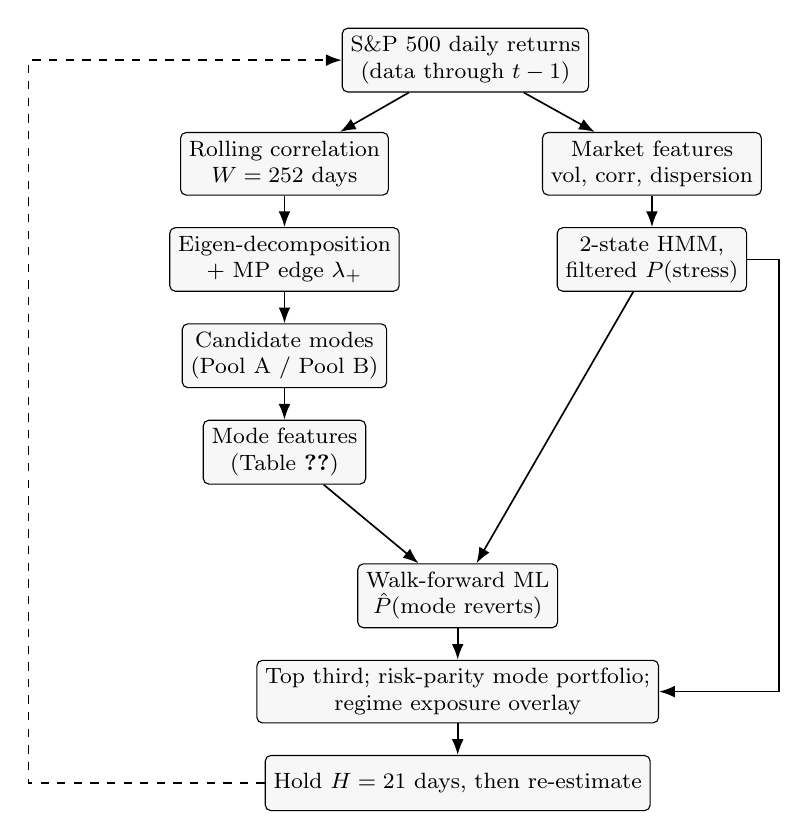
\begin{tikzpicture}[
  node distance=4mm and 6mm,
  box/.style={draw, rounded corners=2pt, align=center, font=\footnotesize,
              minimum height=7mm, inner sep=3pt, fill=gray!6},
  arr/.style={-{Latex[length=2mm]}, semithick}]
  \node[box] (ret) {S\&P 500 daily returns\\(data through $t-1$)};
  \node[box, below left=5mm and -6mm of ret] (corr) {Rolling correlation\\$W=252$ days};
  \node[box, below=of corr] (eig) {Eigen-decomposition\\+ MP edge $\lambda_+$};
  \node[box, below=of eig] (modes) {Candidate modes\\(Pool A / Pool B)};
  \node[box, below=of modes] (mf) {Mode features\\(Table~\ref{tab:features})};
  \node[box, below right=5mm and -6mm of ret] (mk) {Market features\\vol, corr, dispersion};
  \node[box, below=of mk] (hmm) {2-state HMM,\\filtered $P(\text{stress})$};
  \node[box, below=10mm of mf, xshift=22mm] (ml) {Walk-forward ML\\$\hat P(\text{mode reverts})$};
  \node[box, below=of ml] (port) {Top third; risk-parity mode portfolio;\\regime exposure overlay};
  \node[box, below=of port] (wf) {Hold $H=21$ days, then re-estimate};
  \draw[arr] (ret) -- (corr);
  \draw[arr] (ret) -- (mk);
  \draw[arr] (corr) -- (eig);
  \draw[arr] (eig) -- (modes);
  \draw[arr] (modes) -- (mf);
  \draw[arr] (mk) -- (hmm);
  \draw[arr] (mf) -- (ml);
  \draw[arr] (hmm) -- (ml);
  \draw[arr] (hmm.east) -- ++(4mm,0) |- (port.east);
  \draw[arr] (ml) -- (port);
  \draw[arr] (port) -- (wf);
  \draw[arr, dashed] (wf.west) -- ++(-30mm,0) |- (ret.west);
\end{tikzpicture}
\caption{Pipeline. Each arrow uses only information available at the
close before the episode starts. The dashed arrow marks the monthly
walk-forward step.}
\label{fig:pipeline}
\end{figure}


\paragraph{Data.} We use daily dividend- and split-adjusted closing
prices from Yahoo Finance for the \DataAssets{} current S\&P~500
constituents with a complete price history from \DataStart{} to
\DataEnd{} (\DataDays{} trading days of log returns). Restricting to
current constituents with full histories introduces survivorship bias
(Section~\ref{sec:limitations}). Interior gaps of up to five days are
forward-filled; no other cleaning is applied.

\paragraph{Episodes.} \Cref{fig:pipeline} summarizes the pipeline. The walk-forward is organized in \emph{episodes}.
At re-estimation day $t$, the correlation matrix is estimated on the
trailing window $[t-W,t)$ with $W=252$. Its eigenvectors and the asset
volatilities $\sigma_i$ are frozen and traded over the holding period
$[t,t+H)$ with $H=21$. The holding period equals the re-estimation step,
so the episodes tile the sample without overlap: there are
\NEpisodes{} episodes from January~2011. Everything recorded about the
estimation window (features) uses data strictly before $t$, and
everything recorded about the holding period (labels, PnL) uses data
from $t$ on. Because episode $i$'s label is fully realized when episode
$i+1$ begins, a model trained on episodes $<j$ can score episode $j$
with no overlap between training labels and test data.

\paragraph{Signal.} On each trading day $d$ of an episode, mode $k$'s
position is the negative, clipped $z$-score of its cumulative price
relative to the previous $L=60$ days,
\begin{equation}
  s_{k,d} = -\operatorname{clip}\!\left(
    \frac{X_{k,d-1}-\bar X_{k}^{(L)}}{\operatorname{sd}(X_{k})^{(L)}},\,-3,\,3\right),
  \label{eq:signal}
\end{equation}
where the mean and standard deviation are taken over days $d-L,\dots,d-1$.
This bets that a displaced normal coordinate is pulled back toward its
recent equilibrium. The original specification in the code repository,
a $z$-score of the daily mode \emph{return} over 20 days, is a
short-term reversal bet; we report it for comparison.

\paragraph{Label.} The standalone forward PnL of mode $k$ in an episode
is $\pi_k=\sum_{d=t}^{t+H-1}s_{k,d}\,r_{k,d}$. The binary label is
$y_k=\mathbf 1\{\pi_k>0\}$: did trading the mode's reversion signal make
money over the next month? This ties ``mean reversion'' directly to the
quantity a strategy can monetize. As a purely statistical check we
also report the out-of-sample lag-1 autocorrelation of mode returns.

\paragraph{Candidate pools.} Mode~0 is the market mode in every window
(its overlap with the normalized equal-weight vector is
\FullOverlap{} in the full sample) and is never a candidate. We fixed
\emph{Pool~A}, modes $1$--$30$, before seeing any out-of-sample
result. It contains all signal modes ($n_s$ ranges from 3 to 11 across
episodes) plus the first part of the noise bulk, and so lets the models
learn whether the MP edge matters. \emph{Pool~B}, every non-degenerate
mode ($1$--$249$), was added after the spectrum-wide test in
Section~\ref{sec:spectrum}; results on Pool~B should be read with that
in mind.

\section{Predicting which modes revert}
\label{sec:ml}

\subsection{Features}

Every feature is computed from the estimation window only.
Table~\ref{tab:features} lists them by group. The groups follow the
mechanisms discussed above: eigenvalue position (where the mode sits
relative to the MP edge and its neighbours), estimated speed of
reversion, serial dependence, eigenvector stability (whether the mode
is the ``same'' portfolio from one month to the next), volatility
regime of the mode, and portfolio concentration (whether the mode is a
broad combination or a near-pair). We add the mode's trailing
in-window reversion performance and, for the regime-aware models, the
market-level state described in Section~\ref{sec:regimes}.

\begin{table}[t]
\centering\small
\caption{Mode-level and market-level predictors. All are computed on the
estimation window $[t-W,t)$ or, for regime variables, from data through
the close of day $t-1$.}
\label{tab:features}
\begin{tabular}{@{}llp{8.4cm}@{}}
\toprule
Group & Feature & Definition \\
\midrule
Eigenvalue & \texttt{mode\_index} & rank $k$ \\
separation & \texttt{lam\_over\_mp} & $\lambda_k/\lambda_+$ \\
 & \texttt{log\_lambda} & $\log\lambda_k$ \\
 & \texttt{eig\_gap} & $\min(\lambda_{k-1}-\lambda_k,\ \lambda_k-\lambda_{k+1})/\lambda_k$ \\
Half-life & \texttt{log\_half\_life} & $\log$ of $\ln2/(-\ln b)$, $b$ the AR(1) slope of $X_k$ over the window (capped at 252 days) \\
Autocorrelation & \texttt{ac1} & lag-1 autocorrelation of $r_k$ \\
 & \texttt{vr5} & Lo--MacKinlay variance ratio VR(5) of $r_k$ \citep{lomackinlay1988} \\
Stability & \texttt{stability} & $\max_j |v_k^{(t)\top}v_j^{(t-H)}|$ over the previous episode's modes \\
Volatility & \texttt{vol\_ratio} & 21-day volatility of $r_k$ divided by $\sqrt{\lambda_k}$ \\
Concentration & \texttt{participation} & $1/(N\sum_i v_{ik}^4)$, the effective fraction of assets in the mode \\
 & \texttt{max\_weight} & largest $|v_{ik}/\sigma_i|$ as a share of $\sum_i|v_{ik}/\sigma_i|$ \\
Trailing & \texttt{trail\_rev\_sharpe} & Sharpe ratio of the mode's signal \eqref{eq:signal} over the last 63 window days \\
\midrule
Regime & \texttt{p\_stress} & filtered HMM stress probability \\
 & \texttt{log\_vol} & log 21-day realized volatility of the equal-weight market \\
 & \texttt{avg\_corr} & 63-day average pairwise correlation \\
 & \texttt{absorption} & $\lambda_0/N$, share of variance in the market mode \citep{kritzman2011} \\
\bottomrule
\end{tabular}
\end{table}

\subsection{Models and protocol}

We compare an $\ell_2$-regularized logistic regression ($C=0.1$, features
standardized), histogram gradient boosting (depth~3, 150 iterations,
learning rate 0.05, minimum leaf size 50), and a random forest (300
trees, minimum leaf size 25). Hyperparameters were set once to
conservative values and not tuned. We pre-specified the logistic model
as primary because the signal-to-noise ratio of the problem is low.
Models are trained on an expanding window of all (episode, mode) rows
from episodes $<j$ and score episode~$j$. The first prediction is made
after \MinTrain{} episodes (about two years), so the out-of-sample
period starts on \OOSStart{}. The logistic model is re-fit every
episode and the tree ensembles every third episode. We report the
out-of-sample AUC with 95\% confidence intervals from a bootstrap that
resamples whole episodes, which respects the cross-sectional
dependence among modes in the same month.

\section{Market regimes}
\label{sec:regimes}

Statistical-arbitrage returns are known to depend on the market
environment. Reversion profits are typically higher when dispersion is
high, and they can collapse in crowded deleveraging episodes
\citep{khandani2011}. We summarize the environment with three daily
features computed from data through day~$d$: the log 21-day realized
volatility of the equal-weight market return; the 63-day average
pairwise correlation; and the log 21-day average cross-sectional return
dispersion. The average correlation is obtained without forming any
matrix. For $N$ unit-variance assets with average correlation
$\bar\rho$, the cross-sectional mean of volatility-standardized returns
has variance $\bar\rho + (1-\bar\rho)/N$, which we invert.

A two-state Gaussian hidden Markov model \citep{hamilton1989} with
diagonal covariances is fit by Baum--Welch \citep{rabiner1989}. To
avoid look-ahead, the model is refit once a year on all data before
1~January, with features standardized using that training set's
moments. The probabilities passed downstream are \emph{filtered}
(forward-algorithm) probabilities $P(\text{stress}\mid x_{1:d})$, never
smoothed ones. States are ordered by mean volatility, so state~1 is
always the high-volatility state, and the stress probability on the
day before an episode starts enters both the ML models (as a feature)
and the portfolio (as an exposure overlay).

\section{Results}
\label{sec:results}

\subsection{The spectrum}
\label{sec:spectrum-desc}

\Cref{fig:spectrum} shows the familiar picture. In the full sample the
market mode carries $\lambda_0=\FullLamZero$, or \FullLamZeroShare\% of
total variance, and its eigenvector is almost exactly the equal-weight
portfolio (overlap \FullOverlap). Once the bulk is rescaled for the
variance absorbed by the market mode \citep{laloux1999}, the remaining
eigenvalues sit close to the Marchenko--Pastur density, with
\FullNSigRescaled{} modes above the edge. In the rolling 252-day windows
($q=\RollQ$) the edge is $\lambda_+=\RollMPUpper$. Between 3 and 11
modes clear it, a handful of sector-like factors behind the market
mode, and everything else is statistically indistinguishable from
noise. (The walk-forward uses the unrescaled, conservative edge with
$\sigma^2=1$. The rescaled edge admits about 13 modes per window, all
inside Pool~A, and changes none of the conclusions below.)

\begin{figure}[t]
\centering
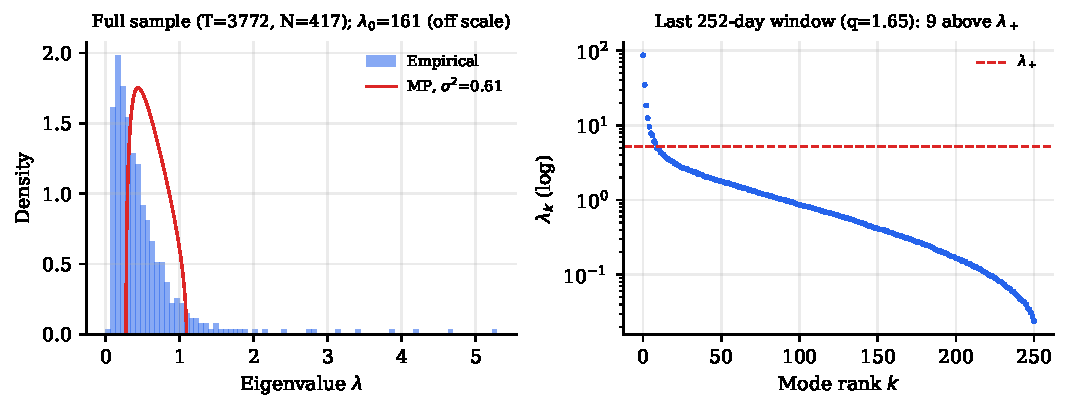
\includegraphics[width=\textwidth]{spectrum}
\caption{Left: full-sample eigenvalue density against the Marchenko--Pastur
law, rescaled for the variance absorbed by the market mode. Right:
eigenvalues of the last 252-day window on a log scale, with the edge
$\lambda_+$ used in the walk-forward. Beyond rank $T-1=251$ the
eigenvalues are exactly zero.}
\label{fig:spectrum}
\end{figure}

\subsection{Where is the mean reversion?}
\label{sec:spectrum}

Our first test uses no machine learning. In every episode we trade the
standalone reversion signal \eqref{eq:signal} on \emph{every}
non-degenerate mode, normalize each mode's PnL by $\sqrt{\lambda_k}$,
and average within buckets defined relative to that episode's own MP
edge $n_s$. \Cref{tab:spectrum} and \cref{fig:spectrum-reversion}
report out-of-sample (2013--2024), pre-cost results.

\begin{table}[t]
\centering\small
\caption{Out-of-sample standalone reversion by position in the spectrum,
2013--2024, before costs. Buckets are defined relative to each episode's
MP edge $n_s$. Sharpe ratios are annualized for an equal-risk portfolio
of the modes in the bucket; $t_{NW}$ uses Newey--West standard errors
with 10 lags. The last two columns give the mean out-of-sample lag-1
autocorrelation of daily mode returns within an episode and its $t$-statistic
across episodes.}
\label{tab:spectrum}
\begin{tabular}{lrrrrrr}
\toprule
 & \multicolumn{2}{c}{Level reversion} & \multicolumn{2}{c}{Return reversal} & \multicolumn{2}{c}{OOS lag-1 AC} \\
\cmidrule(lr){2-3}\cmidrule(lr){4-5}\cmidrule(lr){6-7}
Modes & Sharpe & $t_{NW}$ & Sharpe & $t_{NW}$ & $\bar\rho_1$ & $t$ \\
\midrule
Market ($k=0$) & -0.09 & -0.33 & 0.18 & 0.56 & -0.066 & -4.06 \\
Signal, above MP ($1..n_s-1$) & 0.07 & 0.26 & -0.57 & -1.96 & -0.047 & -6.33 \\
Edge bulk ($n_s..n_s+24$) & -0.00 & -0.02 & -0.25 & -0.71 & -0.054 & -12.05 \\
Upper bulk ($n_s+25..99$) & 0.54 & 1.86 & 0.63 & 2.89 & -0.057 & -21.71 \\
Middle bulk ($100..174$) & 0.87 & 2.74 & 1.10 & 4.07 & -0.057 & -21.66 \\
Lower bulk ($175..249$) & 0.70 & 2.39 & 0.95 & 3.14 & -0.056 & -22.15 \\
\bottomrule
\end{tabular}
\end{table}

\begin{figure}[t]
\centering
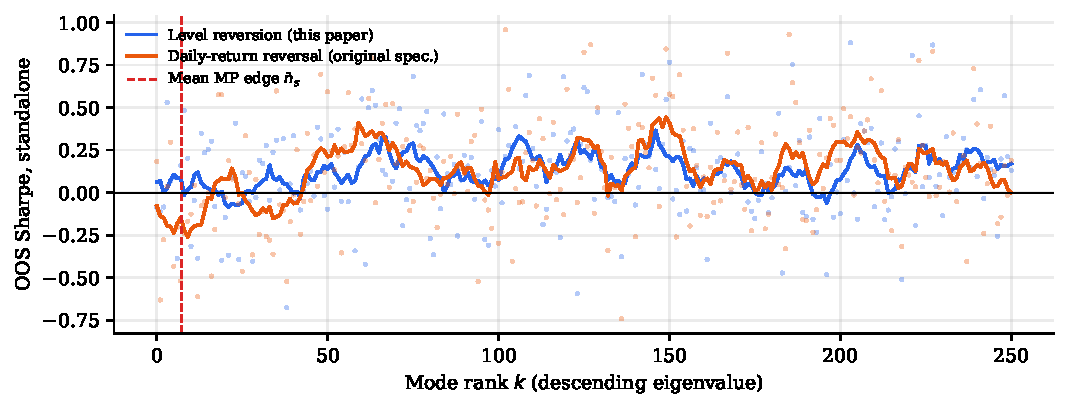
\includegraphics[width=\textwidth]{spectrum_reversion}
\caption{Out-of-sample Sharpe ratio of the standalone reversion signal for
each mode rank (dots) and a 9-mode moving average (lines), 2013--2024,
before costs. The dashed line marks the average MP edge.}
\label{fig:spectrum-reversion}
\end{figure}

Three results stand out.

\emph{First, the modes that random matrix theory certifies as signal do
not mean-revert in a tradable way.} The level-reversion Sharpe ratio of
the above-MP modes is \SRSignalLevel{} ($t=\TSignalLevel$). For the
first 25 modes below the edge it is \SREdgeLevel{}. The original
repository's daily-return reversal signal does worse on the signal
modes (\SRSignalRet, $t=\TSignalRet$): these portfolios are sector-like
factors that trend over days rather than revert.

\emph{Second, reversion lives in the bulk.} The Sharpe ratio rises to
\SRUpperLevel{} for modes $n_s+25$ to 99, \SRMiddleLevel{} for modes
100--174 ($t=\TMiddleLevel$) and \SRLowerLevel{} for the lowest modes
($t=\TLowerLevel$). The same pattern, slightly stronger, holds for the
return-reversal signal (\SRMiddleRet, $t=\TMiddleRet$). Purely
statistically, every bucket has negative out-of-sample lag-1
autocorrelation. For the market and signal modes it is about $-0.05$
($t\approx\ACtSignal$), and in the bulk it is about \ACMiddle{} with
$t$-statistics above 20 in absolute value. Mode returns at the bottom
of the spectrum reverse day to day, as the overdamped picture of
\cref{sec:theory} suggests. The reversal is economically small: a lag-1
autocorrelation of $-0.06$ explains well under 1\% of next-day variance.

\emph{Third, the simple OU prediction for half-lives fails.}
Equation~\eqref{eq:prediction} predicts that the in-window half-life
rises one-for-one with $\lambda_k$ on a log scale. The fitted slope
across all modes and episodes is \OUSlope{}, and the Spearman correlation
is \OUSpearman{} (\cref{fig:ou} in the appendix). The 252-day AR(1)
half-life of the level is a poor statistic for day-scale reversal, and
the lowest-variance sample eigenvectors are partly artefacts of
estimation noise, whose in-sample variance is biased downward
\citep{bunbouchaud2017}. The qualitative ordering of
\eqref{eq:equipartition}, with stiff directions reverting faster, shows
up in out-of-sample \emph{profitability}, not in in-sample half-lives.

These findings reframe the original thesis. The intuition that the
``smallest signal modes'' are the natural building blocks of a reversion
portfolio is right about direction (small eigenvalues) but wrong about
where to stop. The MP filter discards exactly the part of the spectrum
where reversion is concentrated.

\subsection{Can mode quality be predicted?}
\label{sec:ml-results}

The base rate is high, with \BaseRateA\% of Pool~A mode-months
profitable out of sample. This reflects the negative skew of reversion
payoffs: many small gains and occasional large losses. \Cref{tab:auc}
reports out-of-sample AUCs.

\begin{table}[t]
\centering\small
\caption{Out-of-sample AUC for predicting $y=\mathbf 1\{\pi_k>0\}$,
2013--2024 (\OOSRowsA{} mode-months in Pool~A, \OOSRowsB{} in Pool~B).
Brackets: 95\% intervals from a bootstrap over episodes. Heuristics
rank modes by a single in-window statistic.}
\label{tab:auc}
\begin{tabular}{llcc}
\toprule
Pool & Model & Mode features & Mode + regime features \\
\midrule
Modes 1--30 & Logistic (L2) & 0.523 [0.506, 0.540] & 0.521 [0.501, 0.537] \\
 & Gradient boosting & 0.518 [0.502, 0.535] & 0.518 [0.499, 0.538] \\
 & Random forest & 0.524 [0.508, 0.543] & 0.528 [0.509, 0.545] \\
 & Heuristic: $-\log$ half-life & \multicolumn{2}{c}{0.512} \\
 & Heuristic: $-\log\lambda$ & \multicolumn{2}{c}{0.504} \\
\midrule
Full spectrum & Logistic (L2) & 0.508 [0.500, 0.515] & 0.514 [0.505, 0.522] \\
 & Gradient boosting & 0.506 [0.501, 0.512] & 0.504 [0.497, 0.512] \\
 & Random forest & 0.507 [0.500, 0.513] & 0.512 [0.505, 0.520] \\
 & Heuristic: $-\log$ half-life & \multicolumn{2}{c}{0.512} \\
 & Heuristic: $-\log\lambda$ & \multicolumn{2}{c}{0.493} \\
\bottomrule
\end{tabular}
\end{table}

\begin{table}[t]
\centering\small
\caption{Feature-group importance for the primary (logistic, all-feature)
model. ``Solo AUC'' trains on that group alone; ``$\Delta$AUC (drop)''
is the change in out-of-sample AUC when the group is removed.}
\label{tab:ablation}
\begin{tabular}{lrrrr}
\toprule
 & \multicolumn{2}{c}{Modes 1--30} & \multicolumn{2}{c}{Full spectrum} \\
\cmidrule(lr){2-3}\cmidrule(lr){4-5}
Feature group & Solo AUC & $\Delta$AUC (drop) & Solo AUC & $\Delta$AUC (drop) \\
\midrule
Eigenvalue separation & 0.504 & +0.003 & 0.507 & -0.001 \\
Half-life & 0.510 & +0.002 & 0.508 & -0.001 \\
Autocorrelation & 0.522 & -0.004 & 0.501 & +0.001 \\
Eigenvector stability & 0.506 & -0.000 & 0.498 & +0.000 \\
Volatility & 0.512 & -0.002 & 0.491 & +0.000 \\
Concentration & 0.523 & -0.005 & 0.490 & -0.001 \\
Trailing reversion & 0.511 & +0.001 & 0.497 & +0.000 \\
Regime & 0.506 & +0.002 & 0.512 & -0.006 \\
\bottomrule
\end{tabular}
\end{table}

Predictability is real but small. In Pool~A every model clears 0.5. The
logistic model with mode features reaches \AUCLogitModeA{}
[\AUCLoLogitModeA, \AUCHiLogitModeA], and the random forest with all
features reaches \AUCRfAllA{} [\AUCLoRfAllA, \AUCHiRfAllA]. Gradient
boosting is no better than the linear model, as expected when the
signal-to-noise ratio is this low. In Pool~B, where most rows are bulk
modes that all revert to a similar degree, the AUCs fall to 0.504--0.514.
The single-statistic heuristics score below the multivariate models:
ranking by short half-life gives \AUCHeurHalfLifeA{} in Pool~A, and
ranking by small eigenvalue gives \AUCHeurLambdaA, indistinguishable
from chance.

The ablation in \cref{tab:ablation} shows no single dominant group.
The most informative groups on their own are portfolio concentration
(broad modes revert more reliably than near-pairs) and autocorrelation;
removing any one group changes the AUC by less than 0.006. Adding the
regime features barely changes the AUC, but it does change the
\emph{level} of predicted probabilities. In Pool~A the base rate is
\BaseRateAStress\% in the stress state against \BaseRateACalm\% in the
calm state, and the mean normalized forward PnL is negative in calm
months. Timing, rather than cross-sectional selection, is where the
regime information pays off (\cref{sec:strategy}).

\begin{figure}[t]
\centering
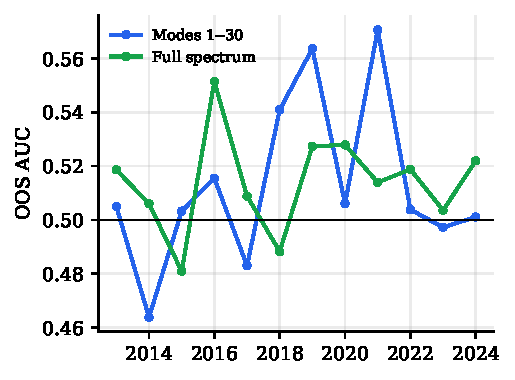
\includegraphics[width=0.5\textwidth]{auc_by_year}
\caption{Out-of-sample AUC by calendar year for the primary model.}
\label{fig:auc-year}
\end{figure}

\begin{figure}[t]
\centering
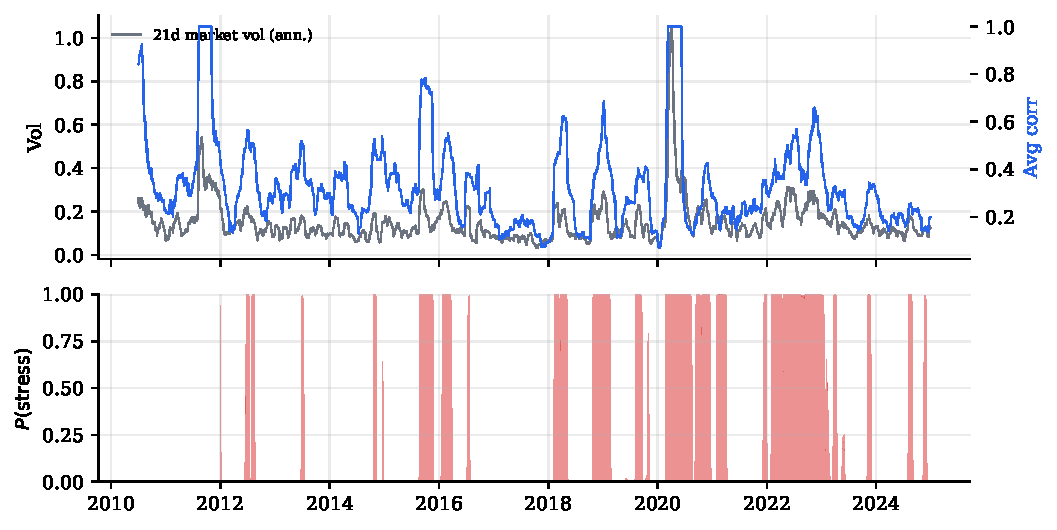
\includegraphics[width=\textwidth]{regimes}
\caption{Regime features (top) and the walk-forward filtered stress
probability (bottom).}
\label{fig:regimes}
\end{figure}

\subsection{Regimes}

The two HMM states are cleanly separated
(\cref{fig:regimes}). In the most recent fit, the calm state
has \CalmVol\% annualized market volatility and an average pairwise
correlation of \CalmCorr, against \StressVol\% and \StressCorr{} in the
stress state. Both states are persistent (daily stay probabilities
\PStayCalm{} and \PStayStress). The filtered stress probability exceeds
one half on \FracStress\% of days: \StressTwentyTwenty\% of 2020,
\StressTwentyTwentyTwo\% of 2022 and \StressTwentySeventeen\% of 2017.

\subsection{Walk-forward strategies}
\label{sec:strategy}

\paragraph{Construction.} In each episode the selected modes are traded
with signal \eqref{eq:signal}, each scaled by $1/\sqrt{\lambda_k}$ for equal
ex-ante risk. Mode positions are mapped to asset weights
$x_i=\sum_k w_k\,s_k\,v_{ik}/(\sqrt{\lambda_k}\sigma_i)$ and rescaled
daily to unit gross exposure. ML strategies select the top third of
each episode's pool by predicted probability. Costs are 2~bp per unit
of one-way turnover. All strategies are evaluated on the same period
(7 January 2013 -- 30 December 2024).

\paragraph{Regime overlay.} The episode-level exposure is
$e_j=(1-p_j)g_{\text{calm}}+p_j g_{\text{stress}}$, where $p_j$ is the
filtered stress probability before the episode and
$g_s=\operatorname{clip}(\widehat{SR}_s/\max_{s'}\widehat{SR}_{s'},0,1)$.
Here $\widehat{SR}_s$ is the strategy's own past gross Sharpe ratio on
days classified to regime $s$, using only completed episodes. The best
regime so far is traded at full size and a regime with a negative past
Sharpe is not traded. \emph{Disclosure:} our pre-specified overlay could
only de-risk in the stress state. It was never active, because the
strategy's past stress-state Sharpe always exceeded its calm-state
Sharpe. The symmetric rule above replaced it after we saw this. The
rule is still strictly walk-forward, but its form was informed by the
data, and its results should be discounted accordingly.

\begin{table}[t]
\centering\small
\caption{Walk-forward strategy performance, 7 January 2013 -- 30 December 2024. Net of
2~bp per unit turnover unless labelled gross. Turnover is average daily
one-way turnover as a fraction of gross exposure. Break-even is the
cost in bp per unit turnover at which the net return is zero.}
\label{tab:strategies}
\resizebox{\textwidth}{!}{\begin{tabular}{llrrrrrrr}
\toprule
Strategy & Pool & Ann. ret. & Ann. vol & Sharpe & Gross SR & Max DD & Turnover & Break-even \\
\midrule
Original repo specification & -- & -10.5\% & 6.9\% & -1.53 & -0.53 & -125.8\% & 1.36 & -1.06 \\
\midrule
MP signal modes, equal weight & 1--30 & -0.7\% & 5.2\% & -0.14 & 0.11 & -20.2\% & 0.26 & 0.88 \\
All candidates, equal weight & 1--30 & -0.8\% & 3.8\% & -0.20 & 0.16 & -22.7\% & 0.27 & 0.88 \\
Heuristic: shortest half-life & 1--30 & -1.1\% & 2.5\% & -0.46 & 0.14 & -15.1\% & 0.30 & 0.47 \\
ML: mode features & 1--30 & -0.8\% & 2.7\% & -0.29 & 0.24 & -15.7\% & 0.29 & 0.91 \\
ML: mode + regime features & 1--30 & -1.3\% & 2.5\% & -0.50 & 0.07 & -15.2\% & 0.29 & 0.25 \\
ML + regime + exposure overlay & 1--30 & -0.4\% & 2.0\% & -0.21 & 0.18 & -9.2\% & 0.15 & 0.93 \\
Equal weight + exposure overlay & 1--30 & -0.3\% & 3.2\% & -0.09 & 0.14 & -14.4\% & 0.14 & 1.26 \\
\midrule
All candidates, equal weight & Full & -0.3\% & 2.2\% & -0.14 & 0.81 & -10.7\% & 0.42 & 1.70 \\
Heuristic: shortest half-life & Full & -1.1\% & 1.6\% & -0.67 & 0.67 & -13.0\% & 0.43 & 1.00 \\
ML: mode features & Full & -0.5\% & 1.9\% & -0.25 & 0.74 & -11.6\% & 0.37 & 1.50 \\
ML: mode + regime features & Full & -0.2\% & 1.9\% & -0.12 & 0.85 & -10.8\% & 0.36 & 1.76 \\
ML + regime + exposure overlay & Full & 0.3\% & 1.6\% & 0.19 & 0.95 & -6.7\% & 0.24 & 2.49 \\
Equal weight + exposure overlay & Full & 0.3\% & 1.9\% & 0.16 & 0.89 & -6.2\% & 0.28 & 2.44 \\
\bottomrule
\end{tabular}}
\end{table}

\begin{figure}[t]
\centering
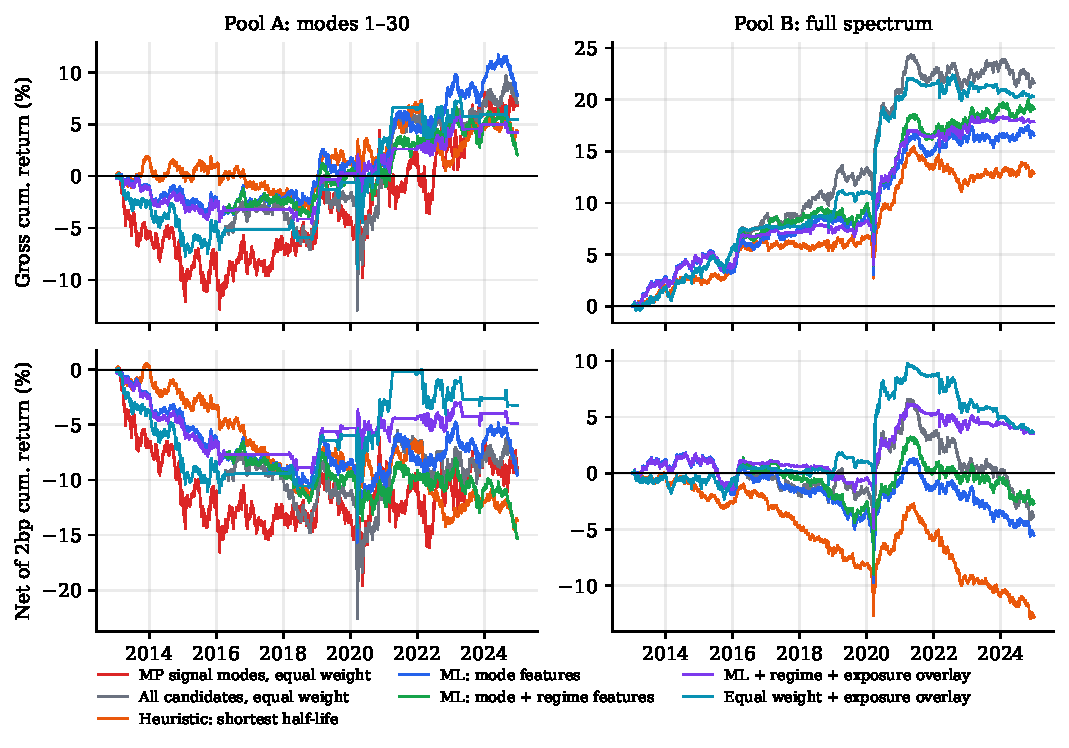
\includegraphics[width=\textwidth]{cumulative_pnl}
\caption{Cumulative log returns per unit gross exposure, before (top) and
after (bottom) 2~bp costs.}
\label{fig:pnl}
\end{figure}

\paragraph{The original specification fails.} The original repository
strategy (daily-return reversal on the top 20 signal modes, raw-return
projection) has a gross Sharpe of \GSROrig{}. With daily turnover of
\TOOrig{} times its book it loses heavily after costs (net Sharpe
\SROrig). Its failure is predicted by \cref{tab:spectrum}: it trades the
part of the spectrum that does not revert, with a signal that is
negative there.

\paragraph{Gross reversion is real, but small relative to turnover.}
Trading every Pool~B mode with equal risk earns a gross Sharpe of
\GSREWB{}, and does so with almost no market exposure. Per unit of gross
exposure, however, the return is only \GRetEWB\% a year against daily
turnover of \TOEWB, a break-even cost of \BEEWB~bp. At 2~bp the net
Sharpe is \SREWB. Pool~A is weaker throughout (gross \GSREWA). The
long-short book is extremely diversified, so its volatility per unit
gross is low (\VolEWB\%), and a levered implementation would scale return
and volatility together. Costs, not risk, are the binding constraint.

\paragraph{ML selection beats random selection, not diversification.}
In Pool~B, the ML-selected top third has a gross Sharpe of
\GSRMLAllB{}. A randomly selected top third of the same size averages
\PlaceboMeanB{} net (95th percentile \PlaceboNFB), and the ML strategy
beats every one of 200 random draws ($p<0.005$). But the ML strategy
does not beat simply trading all candidates. The Sharpe difference
against equal weight is \DiffMLAllB{} (bootstrap $p=\DiffPMLAllB$), and in
Pool~A it is negative (\DiffMLAllA). Holding all modes diversifies
away more noise than a weak classifier can add by choosing among them.
The half-life heuristic is significantly \emph{worse} than equal weight
in Pool~B (\DiffHeurB, $p$ for improvement $=\DiffPHeurB$).

\paragraph{Regimes matter most.} Reversion makes money in the stress
state and loses in the calm state, for every strategy and both pools.
For the Pool~B equal-weight portfolio the Sharpe ratio is
\RegSREWBStress{} in stress and \RegSREWBCalm{} in calm. This matches
the evidence that short-term reversal profits are a compensation for
liquidity provision that rises with volatility
\citep{nagel2012,khandani2011}. The overlay, which learns this
asymmetry walk-forward, raises the net Sharpe of the equal-weight Pool~B
portfolio to \SREWOverB{} (difference \DiffEWOverB, $p=\DiffPEWOverB$).
Combined with ML selection it reaches \SRMLOverB{} (\DiffMLOverB,
$p=\DiffPMLOverB$) and reduces the maximum drawdown from \DDEWB\% to
\DDMLOverB\%. Part of the gain comes from lower turnover, since the
overlay often trades at reduced size. The gross Sharpe also rises, to
\GSRMLOverB.

\subsection{Robustness}
\label{sec:robustness}

\begin{figure}[t]
\centering
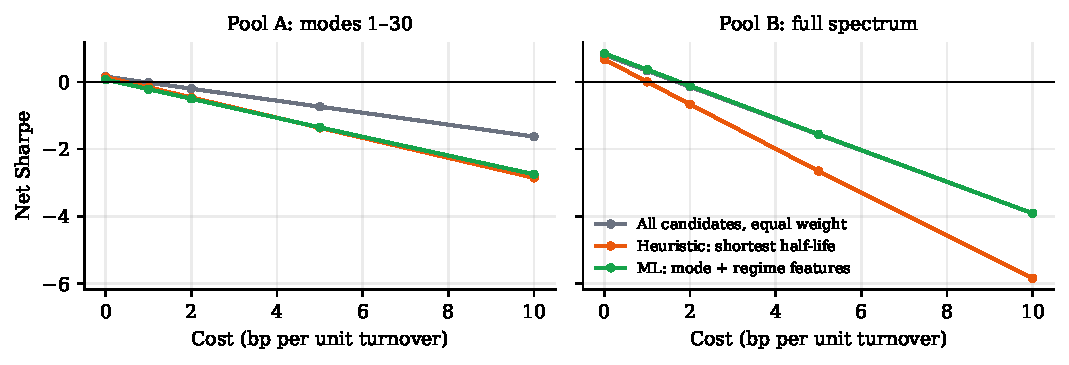
\includegraphics[width=\textwidth]{costs}
\caption{Net Sharpe ratio as a function of the cost per unit turnover.}
\label{fig:costs}
\end{figure}

\begin{table}[t]
\centering\small
\caption{Robustness of the primary ML strategy (logistic, mode + regime
features, top third, no overlay) and the equal-weight benchmark. Net
Sharpe at 2~bp, with gross Sharpe in parentheses. Rows below the rule
re-build the episodes and re-train the models; sub-period rows split
the baseline run.}
\label{tab:robustness}
\resizebox{\textwidth}{!}{\begin{tabular}{lrrrrrr}
\toprule
 & \multicolumn{3}{c}{Pool A: modes 1--30} & \multicolumn{3}{c}{Pool B: full spectrum} \\
\cmidrule(lr){2-4}\cmidrule(lr){5-7}
Test & ML & EW & AUC & ML & EW & AUC \\
\midrule
Baseline ($W$=252, $L$=60, $H$=21) & -0.50 (0.07) & -0.20 (0.16) & 0.521 & -0.12 (0.85) & -0.14 (0.81) & 0.514 \\
\midrule
Sub-period 2013--2016 & -1.27 (-0.42) & -0.92 (-0.37) & -- & 0.04 (1.48) & 0.04 (1.61) & -- \\
Sub-period 2017--2019 & -0.20 (0.51) & -0.29 (0.23) & -- & -0.74 (0.66) & -0.34 (1.05) & -- \\
Sub-period 2020--2021 & -0.05 (0.34) & 0.30 (0.52) & -- & 0.44 (1.03) & 0.56 (1.09) & -- \\
Sub-period 2022--2024 & -0.65 (-0.11) & -0.19 (0.19) & -- & -0.49 (0.47) & -1.20 (-0.12) & -- \\
Select top 20\% & -0.63 (-0.04) & -0.20 (0.16) & -- & -0.25 (0.82) & -0.14 (0.81) & -- \\
Select top 50\% & -0.42 (0.07) & -0.20 (0.16) & -- & -0.08 (0.85) & -0.14 (0.81) & -- \\
Model: GBM & -0.65 (-0.16) & -0.20 (0.16) & -- & -0.56 (0.41) & -0.14 (0.81) & -- \\
Model: RF & -0.36 (0.15) & -0.20 (0.16) & -- & -0.54 (0.64) & -0.14 (0.81) & -- \\
Execution delay +1 day & -0.53 (0.01) & -0.27 (0.10) & 0.514 & -0.74 (0.33) & -0.59 (0.42) & 0.508 \\
Window $W=126$ & -0.60 (-0.01) & -0.24 (0.15) & 0.521 & -0.63 (0.35) & -0.28 (0.36) & 0.516 \\
Window $W=504$ & -0.58 (-0.10) & -0.10 (0.24) & 0.510 & -0.13 (0.87) & -0.31 (0.83) & 0.519 \\
Lookback $L=20$ & -0.70 (0.19) & -0.43 (0.24) & 0.507 & -0.97 (0.64) & -0.36 (0.97) & 0.513 \\
Lookback $L=120$ & -0.66 (-0.13) & -0.21 (0.03) & 0.519 & -0.82 (0.55) & -0.13 (0.60) & 0.521 \\
Holding $H=10$ & -0.31 (0.45) & -0.07 (0.30) & 0.524 & -1.22 (0.64) & -0.44 (0.72) & 0.518 \\
Holding $H=42$ & -0.35 (0.17) & -0.26 (0.09) & 0.510 & -0.24 (0.63) & -0.12 (0.66) & 0.517 \\
\bottomrule
\end{tabular}}
\end{table}

\Cref{fig:costs,tab:robustness} summarize the sensitivity analysis.
Net results are fragile to costs: at 5~bp every strategy has a clearly
negative Sharpe (Pool~B equal weight: \SRCostFiveEWB), and at zero cost
the Pool~B equal-weight Sharpe is \SRCostZeroEWB. Adding one day of
execution delay roughly halves the gross Sharpe ratio in Pool~B (from
\GSREWB{} to 0.42 for equal weight, and from \GSRMLAllB{} to 0.33 for
ML; \cref{tab:robustness}). A large share of the measured reversion is
therefore a one-day effect, consistent with close-to-close bid--ask bounce and
short-lived liquidity shocks. Strategies that cannot trade at the
close would capture much less of it. In Pool~B the gross Sharpe ratio stays positive in every
re-specification (window, lookback, holding period, selection fraction,
model), but the ML strategy beats equal weight net of costs only in a
few of them (e.g.\ $W=504$ or selecting the top half). In Pool~A gross
Sharpe ratios are near zero throughout. Gross performance is strongest
in 2013--2016 and 2020--2021 and weak in 2022--2024. Gradient boosting
and random forests produce worse strategies than the logistic model,
despite similar AUCs.

\section{Discussion}
\label{sec:discussion}

\paragraph{What the normal-mode analogy gets right.} Taken seriously as
an overdamped, thermally driven system, the coupled-oscillator picture
predicts that the \emph{lowest}-variance eigenportfolios relax fastest.
Out of sample, that ordering holds. Reversion profits and negative
autocorrelation are concentrated at the bottom of the spectrum, and the
market and sector modes at the top trend rather than revert. The
analogy is therefore a useful guide to where to look, and it inverts
the usual PCA habit of treating the leading components as the
interesting ones.

\paragraph{What it gets wrong.} The quantitative prediction, a half-life
proportional to $\lambda_k$, is not supported. The reversion we
measure is mostly a one-day effect that does not survive an extra day
of execution delay. That is more naturally read as liquidity provision
and microstructure noise \citep{lehmann1990,nagel2012} spread over many
small-variance combinations of stocks than as slow relaxation toward an
equilibrium.

\paragraph{The Marchenko--Pastur filter is the wrong filter for this
purpose.} RMT tells us which eigenvalues are distinguishable from noise,
and that is the right question for covariance cleaning
\citep{laloux1999,bunbouchaud2017}. For reversion trading, the relevant
object is the low-variance \emph{subspace}. Individual bulk eigenvectors
are unstable, but projecting onto many of them and trading them together
diversifies away their individual instability. This explains why
equal-weighting the whole bulk beats every selection rule we tried.

\paragraph{Machine learning adds little; timing adds more.} With AUCs of
0.51--0.53, the classifiers do find structure. They are significantly
better than random selection, and stability, concentration and
autocorrelation carry information. But their edge is smaller than the
diversification cost of trading only a third of the pool. Regime
information is more valuable as a \emph{timing} signal for the whole
book than as a feature for ranking modes. The regime asymmetry is
large: reversion is unprofitable in calm markets and profitable in
stressed ones. Our overlay exploits it walk-forward, but its form was
chosen after seeing this asymmetry.

\paragraph{Multiple testing.} We report every strategy and variant we
ran. Across them, the best net Sharpe ratio is below 0.2 over twelve
years, so none would survive a deflated-Sharpe adjustment for the
number of trials \citep{baileylopezdeprado2014}. The robust findings
are the cross-spectrum pattern (\cref{tab:spectrum}), which involves
no selection, and the regime asymmetry, which holds in every
specification.

\section{Limitations}
\label{sec:limitations}

\begin{itemize}
\item \textbf{Survivorship.} The universe is the current S\&P~500
  restricted to stocks with complete 2010--2024 histories (\DataAssets{}
  names). This removes delisted and acquired firms. Survivorship
  typically flatters long-only returns more than market-neutral
  reversion, but it can also understate the tail risk of a reversion
  book, which loses when a stock falls and never comes back.
  Point-in-time constituents (e.g.\ CRSP) would fix this.
\item \textbf{Execution.} Signals use closing prices and are traded at
  the same close. The execution-delay test shows that this assumption
  matters a great deal. The cost model is a flat charge per unit
  turnover, with no market impact, borrow costs or financing.
\item \textbf{Estimation.} We use sample correlations with a fixed
  252-day window. Shrinkage or rotationally invariant estimators
  \citep{bunbouchaud2017}, or eigenvector tracking across windows
  rather than re-estimating from scratch, could make individual modes
  more stable and selection more valuable.
\item \textbf{Label.} The binary profitability label discards magnitude,
  and the payoff is negatively skewed. Regression or quantile targets,
  or a direct portfolio objective, might use the weak signal more
  efficiently.
\end{itemize}

\section{Conclusion}

We set out to test whether the low-eigenvalue normal modes of the
equity correlation matrix mean-revert predictably, and whether
supervised learning and regime detection can turn that into a
statistical-arbitrage strategy. On 417 S\&P~500 stocks over 2013--2024,
out of sample, the answers are as follows. Yes, mode portfolios
mean-revert, but at the bottom of the spectrum rather than in the
Marchenko--Pastur signal modes, and mostly at a one-day horizon. Only
weakly can it be predicted which modes will revert: AUC 0.51--0.53,
better than chance and better than random selection, but not better
than holding everything. Market regimes predict \emph{when} reversion
pays far better than mode features predict \emph{which} modes pay.
After realistic costs, the best walk-forward implementation earns a
small positive Sharpe ratio, \SRMLOverB{}, that depends on a
data-informed overlay and on same-close execution. The
coupled-oscillator analogy is a good map of where reversion lives in
the spectrum. It is not, on this evidence, a source of tradable alpha
for a daily close-to-close strategy.


\bibliographystyle{plainnat}
\bibliography{references}

\appendix
\section{Additional figures}

\begin{figure}[h]
\centering
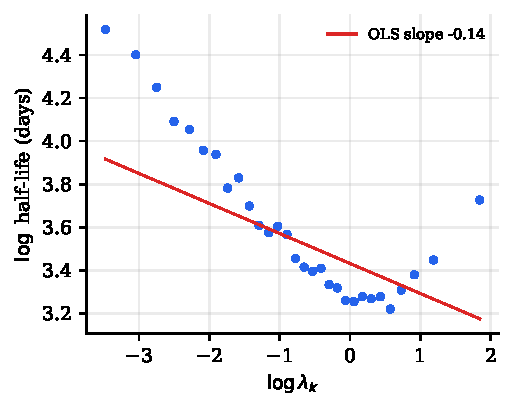
\includegraphics[width=0.48\textwidth]{ou_halflife}
\caption{In-window AR(1) half-life of the cumulative mode price against
$\log\lambda_k$, all modes and episodes (medians in 30 eigenvalue bins).
The OU model \eqref{eq:prediction} predicts slope $+1$; the fitted slope
is \OUSlope. \OUNoRev\% of mode-windows show no detectable reversion
($b\ge1$) and are excluded from the fit.}
\label{fig:ou}
\end{figure}

\begin{figure}[h]
\centering
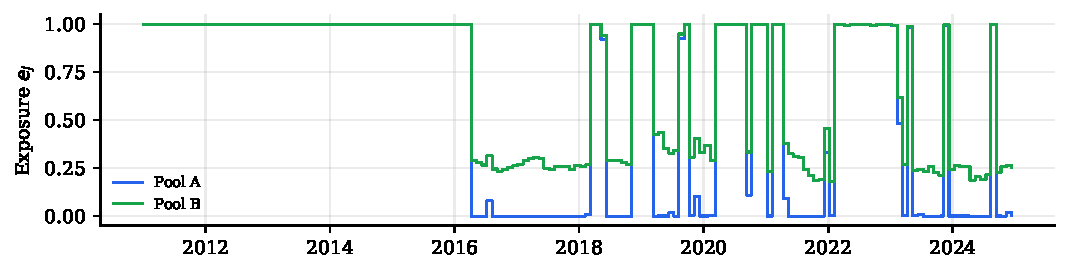
\includegraphics[width=\textwidth]{exposure}
\caption{Walk-forward regime-overlay exposure $e_j$ for the ML strategies.
Average exposure is \MeanExpA{} (Pool~A) and \MeanExpB{} (Pool~B).}
\label{fig:exposure}
\end{figure}


\section{Implementation details}

\paragraph{HMM estimation.} Baum--Welch uses the scaled forward--backward
recursions of \citet{rabiner1989}. It is initialized by splitting the
sample into volatility terciles (halves, for two states), with a
transition matrix of 0.98 on the diagonal, and runs to a log-likelihood
tolerance of $10^{-6}$. Variances are floored at $10^{-4}$ in
standardized units. The first fit uses data from 2010 to 2011 and
produces probabilities from January 2012.

\paragraph{Leakage checks.} The test suite (\texttt{tests/}) perturbs
future data and verifies that nothing computed for the past changes. It
covers the signal, every episode feature, the HMM filter, the
walk-forward HMM refits, and the walk-forward classifier, which is
checked to be invariant to future labels. It also checks that a
single-mode portfolio reproduces the sign of that mode's standalone
PnL, and that the HMM recovers known states on synthetic data.

\paragraph{Reproduction.} \texttt{python scripts/run\_study.py} downloads
the data (cached), runs every stage, and writes all figures and tables
in this paper together with \texttt{output/results.json}.
\texttt{python scripts/make\_macros.py} then regenerates every number
quoted in the text. A full run takes about ten minutes on a laptop.


\end{document}
